\documentclass[12pt,a4paper]{article}

% Margins.
\setlength{\oddsidemargin}{0in}
\setlength{\evensidemargin}{0in}
\setlength{\headheight}{12pt}
\setlength{\headsep}{42pt}
\setlength{\topmargin}{-54pt}
\setlength{\textwidth}{6.5in}
\setlength{\textheight}{10in}

\usepackage{amsmath}
\usepackage{float}
\usepackage{graphicx}
\usepackage[hyphens]{url}
\usepackage{hyperref}	% Clickable links to figures, references and urls.
\usepackage{datetime}
\usepackage{longtable}

% Links direct to top of figures.
\usepackage[all]{hypcap}

% Drawing.
\usepackage{pgf}
\usepackage{tikz}

% Listings for formatting code.
\usepackage{listings}
\usepackage{textcomp}
% General options.
\lstset{breaklines=true, basicstyle=\small\ttfamily, tabsize=4, numbers=left, stepnumber=1, frame=single, showstringspaces=false, upquote=true}
% C++ specific high-lighting. Comments are 50/50 shades of green/black and strings coloured with 60/40 red/black mixture.
\lstset{language=[ISO]C++, commentstyle=\color{green!50!black}, keywordstyle=\color{blue}, stringstyle=\color{red!60!black}}

%opening
\title{\vspace{-2cm}Physics for Engineers\\Class 06\\Introduction to Curvilinear Coordinate Systems}
\author{Attique Dawood}
\date{February 04, 2014\\[0.2cm] Last Modified: \today, \currenttime}
\begin{document}
\maketitle
\section{Announcements}
\begin{itemize}
\item Quiz \#01 today.
\end{itemize}
\section{Revision}
\begin{itemize}
\item Vector product.
\end{itemize}
\section{The Cartesian Coordinate System (2.2S)}
In Cartesian coordinate system the location of a point is expressed in terms of x--, y-- and z--coordinates. A point in Cartesian coordinate system is expressed as (x, y, z). A vector in Cartesian coordinate system has components along $\hat x$, $\hat y$ and $\hat z$.
\begin{equation}
\textbf{A}=A_x\hat x+A_y\hat y+ A_z\hat z.
\end{equation}
The ranges are given by
\begin{equation*}
\begin{split}
&-\infty < x < \infty\\
&-\infty < y < \infty\\
&-\infty < z < \infty\\
\end{split}
\end{equation*}
\section{The Cylindrical Coordinate System (2.3S)}
In Cylindrical coordinate system the location of a point is expressed in terms of $\rho$--, $\phi$-- and z--coordinates. A point in Cylindrical coordinate system is expressed as ($\rho$, $\phi$, z). A vector in Cylindrical coordinate system has components along $\hat \rho$, $\hat \phi$ and $\hat z$.
\begin{equation}
\textbf{A}=A_\rho\hat \rho+A_\phi\hat \phi+ A_z\hat z.
\end{equation}
\begin{figure}[H]
\centering
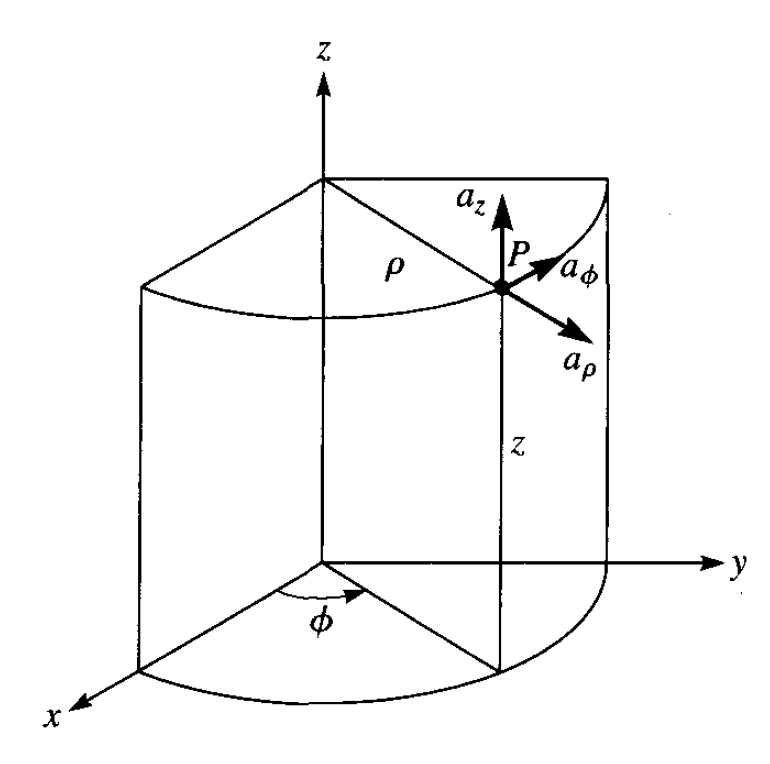
\includegraphics[scale=0.45]{Figure2-1S.png}
\caption{Orientation of unit vectors in Cylindrical coordinates. Figure taken from~\cite[Figure 2.1, page 29]{Sadiku}}
\label{Unit-vectors-cylindrical-coordinates}
\end{figure}
The ranges are given by
\begin{equation*}
\begin{split}
0 < \rho < \infty&\\
0 < \phi < 2\pi&\\
-\infty < z < \infty&\\
\end{split}
\end{equation*}
To convert a point given in Cartesian coordinates following formulas can be used,
\begin{equation}
\begin{split}
&\rho = \sqrt{x^2+y^2}\\
&\phi = \tan^{-1}{\dfrac{y}{x}}
\end{split}
\end{equation}
To convert a point from Cylindrical to Cartesian coordinates,
\begin{equation}
\begin{split}
&x = \rho\cos\phi\\
&y = \rho\sin\phi
\end{split}
\end{equation}
\begin{figure}[H]
\centering
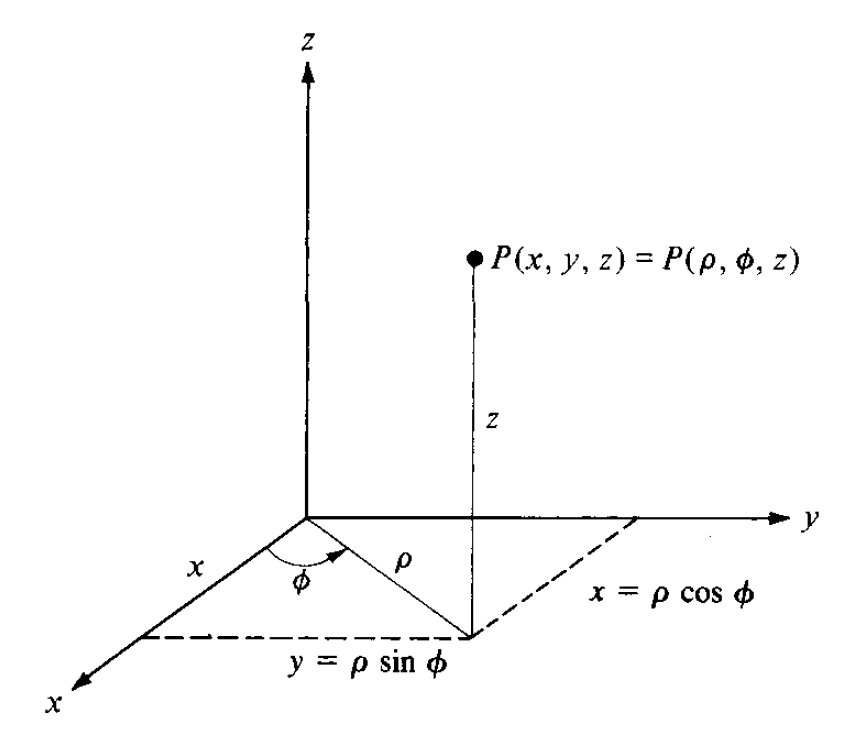
\includegraphics[scale=0.45]{Figure2-2S.png}
\caption{Conversion of point coordinates from Cartesian to Cylindrical. Figure taken from~\cite[Figure 2.2, page 31]{Sadiku}}
\label{Cartesian-to-Cylindrical}
\end{figure}
\section{The Spherical Coordinate System (2.4S)}
In Spherical coordinate system the location of a point is expressed in terms of r--, $\theta$-- and $\phi$. A point in Spherical coordinate system is expressed as (r, $\theta$, $\phi$). A vector in Spherical coordinate system has components along $\hat r$, $\hat \theta$ and $\hat \phi$.
\begin{equation}
\textbf{A}=A_r\hat r+A_\theta\hat \theta+ A_\phi\hat \phi.
\end{equation}
\begin{figure}[htb]
\centering
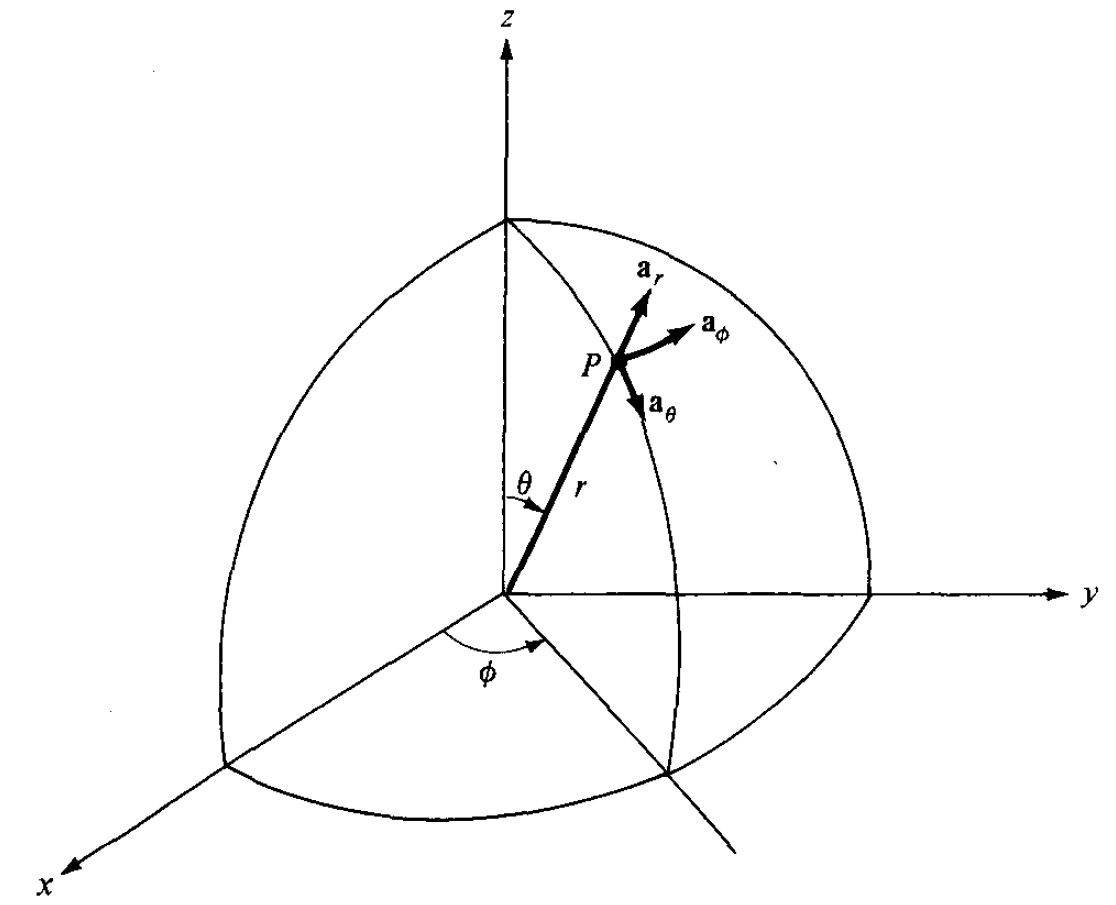
\includegraphics[scale=0.45]{Figure2-4S.png}
\caption{Orientation of unit vectors in Spherical coordinates. Figure taken from~\cite[Figure 2.4, page 33]{Sadiku}}
\label{Unit-vectors-spherical-coordinates}
\end{figure}
The ranges are given by
\begin{equation*}
\begin{split}
0 < r < \infty&\\
0 < \theta < \pi&\\
0 < \phi < 2\pi&\\
\end{split}
\end{equation*}
Conversion formulas for Cartesian and Cylindrical to Spherical are
\begin{equation}
\begin{split}
&r = \sqrt{x^2+y^2+z^2}\\
&\theta = \tan^{-1}{\dfrac{\rho}{z}}=\tan^{-1}{\dfrac{\sqrt{x^2+y^2}}{z}}\\
&\phi = \tan^{-1}{\dfrac{y}{x}}
\end{split}
\end{equation}
Conversion formulas for Spherical to Cylindrical and Cartesian are
\begin{equation}
\begin{split}
&\rho = r\sin\theta\\
&x = r\sin\theta\cos\phi\\
&y = r\sin\theta\sin\phi\\
&z = r\cos\theta
\end{split}
\end{equation}
\begin{figure}[H]
\centering
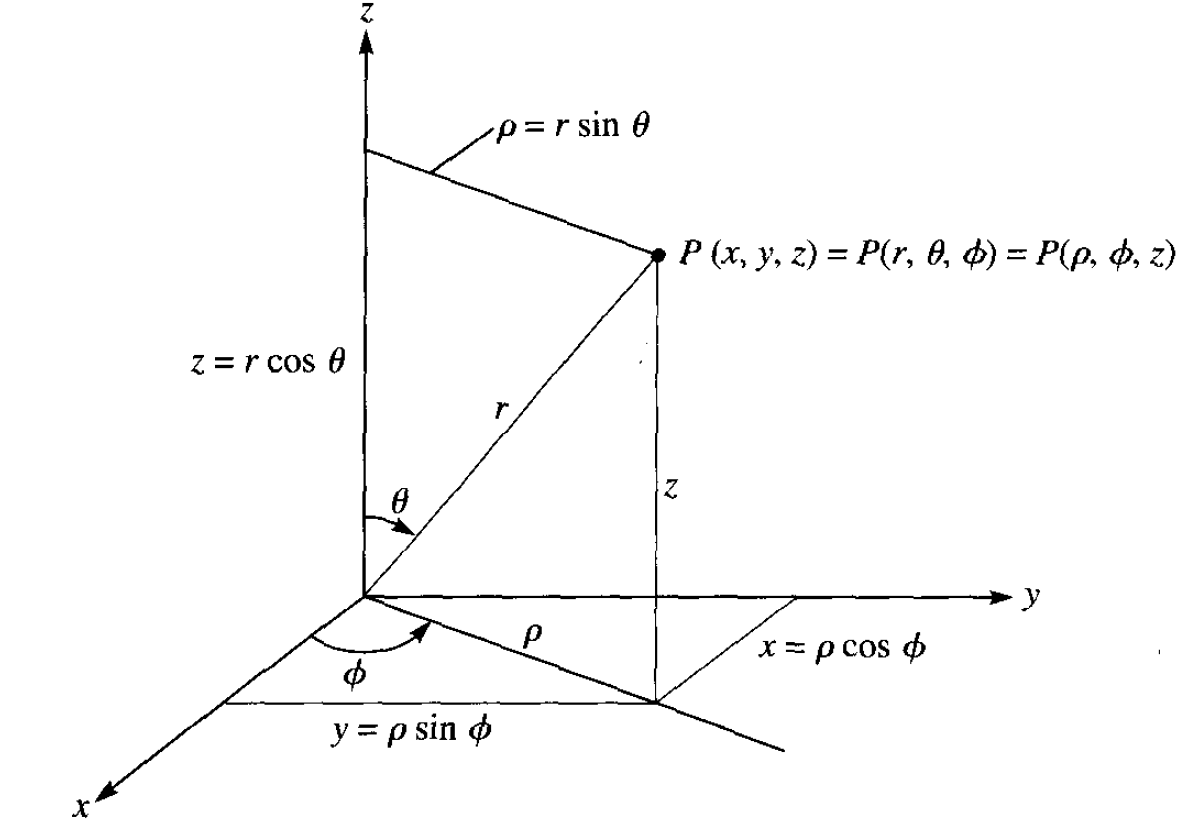
\includegraphics[scale=0.45]{Figure2-5S.png}
\caption{Conversion of point coordinates from Cartesian to Spherical. Figure taken from~\cite[Figure 2.5, page 33]{Sadiku}}
\label{Cartesian-to-Spherical}
\end{figure}
Following relations are useful when using calculator,
\begin{equation*}
\begin{split}
&(\rho, \phi): pol(x,y)\\
&(r, \theta): pol(z, \rho) = pol(z, pol(x, y))\\
&(x, y): rec(\rho, \phi)\\
&(z, \rho): rec(r, \theta)
\end{split}
\end{equation*}
\section{Exercises}
\noindent\textbf{Question 1 (PE 2.1S):} Convert points P(1, 3, 5), T(0, -4, 3), S(-3, -4, -10) to cylindrical and spherical coordinates.
%\nocite{*}
\bibliographystyle{plain}
\bibliography{PhysicsRef}
\end{document}
